\documentclass[12pt,a4paper]{article}
\usepackage[utf8]{inputenc}
\usepackage[T1]{fontenc}

% Packages
\usepackage[margin=1in]{geometry}
\usepackage{graphicx}
\usepackage{hyperref}
\usepackage{listings}
\usepackage{xcolor}
\usepackage{booktabs}
\usepackage{enumitem}
\usepackage{titlesec}
\usepackage{fancyhdr}
\usepackage{array}
\usepackage{multirow}
\usepackage{float}
\usepackage{tikz}
\usetikzlibrary{shapes.geometric, arrows.meta, positioning, fit}

% Hyperref setup
\hypersetup{
    colorlinks=true,
    linkcolor=blue!70!black,
    urlcolor=blue!70!black,
    citecolor=blue!70!black
}

% Code listing style
\lstdefinestyle{cstyle}{
    language=C,
    basicstyle=\ttfamily\small,
    keywordstyle=\color{blue!80!black}\bfseries,
    commentstyle=\color{gray}\itshape,
    stringstyle=\color{orange!80!black},
    numbers=left,
    numberstyle=\tiny\color{gray},
    numbersep=8pt,
    frame=single,
    framesep=4pt,
    breaklines=true,
    tabsize=4,
    showstringspaces=false,
    backgroundcolor=\color{gray!6}
}

\lstdefinestyle{shellstyle}{
    frame=single,
    backgroundcolor=\color{black!85},
    basicstyle=\ttfamily\small\color{white},
    breaklines=true,
    numbers=none
}

% Header / Footer
\pagestyle{fancy}
\fancyhf{}
\rhead{ICS 433 -- Distributed Resource Scheduler}
\lhead{Phase 2 Progress Report}
\rfoot{Page \thepage}

% Title
\title{
    \vspace{-0.5cm}
    \textbf{\large ICS 433 -- Operating Systems} \\[0.4cm]
    \textbf{\LARGE Distributed Resource Scheduler} \\[0.3cm]
    \large Phase 2 Progress Report \\[0.3cm]
    \normalsize King Fahd University of Petroleum \& Minerals
}

\author{
    Rayan Alamri \quad
    Mohammed Alsuhaibani \quad
    Ali Almuzain \quad
    Mohammed Yar
}

\date{April 21, 2026}

% ==============================================================================
\begin{document}
\maketitle
\thispagestyle{fancy}
\tableofcontents
\newpage

% ==============================================================================
\section{Project Recap}

\subsection{Overview}
The Distributed Resource Scheduler is a \textbf{Pure C} system that pools underutilized computing power
across a Local Area Network (LAN) using an asynchronous \textbf{Master--Worker} architecture.
Its goal is to coordinate multiple worker nodes and assign computational tasks efficiently,
demonstrating core OS concepts including multithreading, inter-process communication (IPC),
process isolation, and network socket programming --- all without any external runtime libraries
beyond POSIX and \texttt{pthreads}.

\subsection{Motivation}
Modern distributed systems (e.g., Hadoop, Kubernetes) schedule work across heterogeneous machines.
This project implements a minimal but functionally correct version of such a system in pure C,
targeting POSIX-compliant Unix environments (Linux, macOS, WSL).
The constraints --- no frameworks, no scripting languages --- force direct engagement with
system calls: \texttt{fork()}, \texttt{pipe()}, \texttt{socket()}, \texttt{pthread\_create()},
\texttt{send()}, and \texttt{recv()}.

\subsection{Team Responsibilities}

\begin{center}
\begin{tabular}{ll}
\toprule
\textbf{Team Member} & \textbf{Module} \\
\midrule
Rayan Alamri         & Master Node (server, scheduler, queue, registry) \\
Mohammed Alsuhaibani & Worker Execution Engine (client, executor) \\
Ali Almuzain         & Serialization \& Communication Layer (protocol) \\
Mohammed Yar         & Terminal Dashboard (ncurses UI) \\
\bottomrule
\end{tabular}
\end{center}

% ==============================================================================
\section{What Has Been Implemented}

As of Phase 2, approximately \textbf{75--80\%} of the system is complete.
The networking core, scheduling engine, worker execution pipeline, and serialization
layer are all fully implemented and tested. The terminal dashboard remains as a stub.

\subsection{Master Node (Rayan Alamri) --- 100\% Complete}

\subsubsection{TCP Server (\texttt{src/master/server.c})}
\begin{itemize}[noitemsep]
    \item Binds a \texttt{SOCK\_STREAM} socket on a configurable port (default 9090, overridable via \texttt{MASTER\_PORT} environment variable).
    \item Runs an infinite \texttt{accept()} loop to handle new worker connections.
    \item Validates an initial \texttt{MSG\_REGISTER} handshake before admitting a worker into the registry, preventing random TCP clients from polluting scheduler state.
    \item Spawns a \textbf{detached} \texttt{pthread} per connected worker to receive results and heartbeats concurrently.
    \item On worker disconnection: detects EOF via \texttt{recv\_full()}, requeues any in-flight task, and marks the worker offline.
    \item Includes a demo task seeder thread (activated via \texttt{DEMO\_TASKS} environment variable) that enqueues configurable sample tasks 3 seconds after startup.
\end{itemize}

\subsubsection{Worker Registry (\texttt{src/master/scheduler.c})}
\begin{itemize}[noitemsep]
    \item Fixed-size array of \texttt{WorkerInfo} structs (up to 32 workers, defined by \texttt{MAX\_WORKERS}).
    \item Each entry tracks: \texttt{worker\_id}, \texttt{sock\_fd}, \texttt{status} (\texttt{IDLE}/\texttt{BUSY}/\texttt{OFFLINE}), \texttt{last\_heartbeat} timestamp, and a snapshot of the current task.
    \item All mutations protected by \texttt{pthread\_mutex\_lock()} / \texttt{pthread\_mutex\_unlock()}.
    \item Operations: \texttt{registry\_add()}, \texttt{registry\_set\_status()}, \texttt{registry\_set\_offline()}, \texttt{registry\_find\_idle()}, \texttt{registry\_get()}.
    \item Slot reuse: offline workers free their array index so it can be claimed by new registrations without compacting the table (keeping pointers stable for concurrent readers).
\end{itemize}

\subsubsection{Task Queue (\texttt{src/master/queue\_mgr.c})}
\begin{itemize}[noitemsep]
    \item Dynamically allocated \textbf{FIFO linked list} of \texttt{NetworkPayload} nodes.
    \item Thread-safe via \texttt{pthread\_mutex\_t} + \texttt{pthread\_cond\_t not\_empty}.
    \item Operations: \texttt{queue\_enqueue()}, \texttt{queue\_dequeue()} (blocking), \texttt{queue\_dequeue\_nowait()} (non-blocking), \texttt{queue\_requeue()} (re-inserts at tail), \texttt{queue\_size()}, \texttt{queue\_is\_empty()}, \texttt{queue\_destroy()}.
    \item \texttt{queue\_destroy()} drains all nodes to prevent memory leaks between test runs.
\end{itemize}

\subsubsection{Scheduler Thread (\texttt{src/master/scheduler.c})}
\begin{itemize}[noitemsep]
    \item Runs as a background \texttt{pthread}.
    \item Implements \textbf{Round-Robin} scheduling via a persistent \texttt{rr\_index} cursor over the worker registry.
    \item Uses \texttt{queue\_dequeue\_nowait()} in a polling loop (5\,ms sleep when idle, 10\,ms when no workers are free) to avoid blocking the shutdown path.
    \item Marks a worker \texttt{BUSY} before sending the task; on send failure, requeues the task and marks the worker offline.
    \item Lifecycle: \texttt{scheduler\_init()}, \texttt{scheduler\_start()}, \texttt{scheduler\_stop()} (sets \texttt{running=0} and \texttt{pthread\_join}s the thread).
\end{itemize}

% ------------------------------------------------------------------------------
\subsection{Worker Execution Engine (Mohammed Alsuhaibani) --- 100\% Complete}

\subsubsection{Network Client (\texttt{src/worker/client.c})}
\begin{itemize}[noitemsep]
    \item Connects to the master using \texttt{getaddrinfo()} for DNS resolution and \texttt{IPv4}/\texttt{IPv6} agnosticism.
    \item Accepts host/port/worker-ID via CLI arguments or environment variables (\texttt{MASTER\_HOST}, \texttt{MASTER\_PORT}, \texttt{WORKER\_ID}).
    \item Sends a \texttt{MSG\_REGISTER} handshake immediately after connection.
    \item Spawns a \textbf{heartbeat thread} that sends \texttt{MSG\_HEARTBEAT} packets every 5 seconds; on send failure, shuts down the socket to unblock the main receive loop.
    \item Per-task execution is dispatched to a new \texttt{pthread} so the receive loop remains responsive for concurrent control messages.
    \item Thread-safe sends via a \texttt{send\_lock} mutex (shared between heartbeat and task-result threads).
    \item Graceful shutdown: waits for all in-flight task threads via a condition variable before closing the socket.
\end{itemize}

\subsubsection{Executor (\texttt{src/worker/executor.c})}
\begin{itemize}[noitemsep]
    \item \texttt{executor\_run\_task()} forks a child process for each task, providing CPU isolation.
    \item Uses \texttt{pipe()} for parent--child IPC: the child writes its \texttt{uint32\_t} result and exits; the parent reads it.
    \item Child uses \texttt{\_exit()} to prevent flushing parent-owned \texttt{stdio} buffers.
    \item Parent calls \texttt{waitpid()} after reading the result to reap the child and check its exit status.
    \item Two built-in workloads:
    \begin{itemize}[noitemsep]
        \item \textbf{Command 1 -- Prime Counter:} counts primes up to \texttt{argument} using trial division (avoids \texttt{sqrt()} via \texttt{d <= n/d} to prevent overflow).
        \item \textbf{Command 2 -- Matrix Checksum:} simulates nested-loop CPU work on a virtual matrix of size \texttt{argument}$\times$\texttt{argument} and returns an accumulated checksum.
    \end{itemize}
    \item Error codes: \texttt{EXECUTOR\_OK}, \texttt{EXECUTOR\_ERR\_PIPE}, \texttt{EXECUTOR\_ERR\_FORK}, \texttt{EXECUTOR\_ERR\_CHILD\_IO}, \texttt{EXECUTOR\_ERR\_CHILD\_STATUS}.
\end{itemize}

% ------------------------------------------------------------------------------
\subsection{Serialization \& Communication Layer (Ali Almuzain) --- 100\% Complete}

\subsubsection{Protocol (\texttt{src/shared/protocol.c}, \texttt{src/shared/models.h})}
\begin{itemize}[noitemsep]
    \item \textbf{Fixed-size payload:} all messages use a single \texttt{NetworkPayload} struct (6\,$\times$\,\texttt{uint32\_t} = 24 bytes), eliminating stream fragmentation and variable-length parsing.
    \item \textbf{Byte-order normalization:} \texttt{payload\_to\_net()} converts all fields to network byte order before sending; \texttt{payload\_to\_host()} converts back on receipt --- ensuring cross-architecture compatibility.
    \item \textbf{Reliable I/O:} \texttt{recv\_full()} and \texttt{send\_full()} loop until exactly \texttt{sizeof(NetworkPayload)} bytes have been transferred, handling TCP's byte-stream nature.
    \item \textbf{Message types:} \texttt{MSG\_HEARTBEAT} (0), \texttt{MSG\_TASK} (1), \texttt{MSG\_RESULT} (2), \texttt{MSG\_REGISTER} (3).
    \item \textbf{Worker states:} \texttt{WORKER\_IDLE} (0), \texttt{WORKER\_BUSY} (1), \texttt{WORKER\_OFFLINE} (2).
\end{itemize}

% ------------------------------------------------------------------------------
\subsection{Terminal Dashboard (Mohammed Yar) --- Stub Only}

The dashboard module (\texttt{src/ui/dashboard.c}) currently contains empty stub implementations
for \texttt{dashboard\_init()}, \texttt{dashboard\_run()}, and \texttt{dashboard\_stop()}.
The ncurses-based live monitoring UI is the primary remaining deliverable for Phase 3.

% ------------------------------------------------------------------------------
\subsection{Docker / Deployment Infrastructure}

The following deployment tooling has been added:
\begin{itemize}[noitemsep]
    \item \textbf{Dockerfile} --- multi-stage image for master and worker binaries.
    \item \textbf{docker-compose.yml} --- defines master + worker services with resource limits simulating Raspberry Pi 3/4/5 hardware profiles.
    \item \textbf{scale\_workers.sh} --- launches configurable counts of RPi3/4/5-profile worker containers.
    \item \textbf{manage\_workers.sh} --- add/remove individual containers at runtime to simulate dynamic node join/leave.
    \item \textbf{start-workers.sh} --- convenience script to start N local workers against a given host/port.
\end{itemize}

% ==============================================================================
\section{System Architecture}

\subsection{Component Diagram}

\begin{figure}[H]
\centering
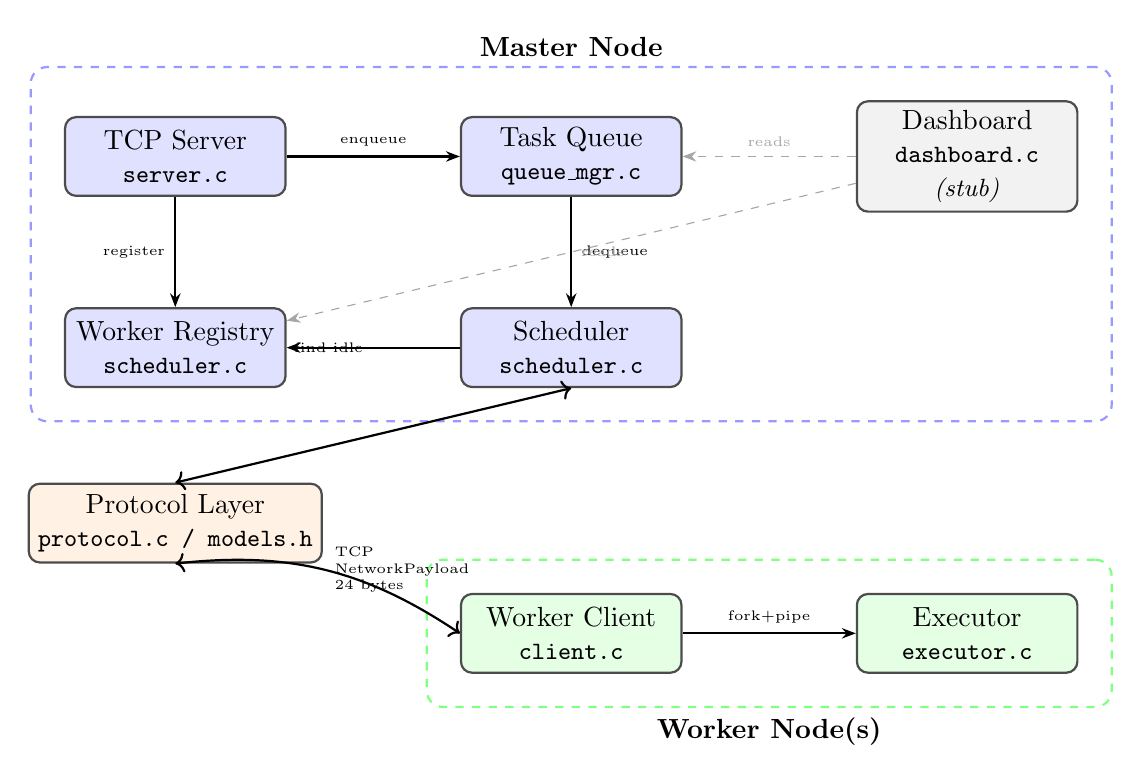
\begin{tikzpicture}[
    node distance=1.4cm and 2.2cm,
    box/.style={rectangle, rounded corners=4pt, draw=black!70, thick,
                minimum width=2.8cm, minimum height=1.0cm,
                align=center, fill=blue!8},
    arrow/.style={-{Stealth[length=5pt]}, thick},
    dasharrow/.style={-{Stealth[length=5pt]}, dashed, gray!70}
]

% Master internals
\node[box, fill=blue!12] (server) {TCP Server\\\small\texttt{server.c}};
\node[box, fill=blue!12, right=2.2cm of server] (queue) {Task Queue\\\small\texttt{queue\_mgr.c}};
\node[box, fill=blue!12, below=1.4cm of queue] (sched) {Scheduler\\\small\texttt{scheduler.c}};
\node[box, fill=blue!12, below=1.4cm of server] (reg) {Worker Registry\\\small\texttt{scheduler.c}};
\node[box, fill=gray!10, right=2.2cm of queue] (dash) {Dashboard\\\small\texttt{dashboard.c}\\\small\textit{(stub)}};

\node[draw=blue!40, dashed, thick, rounded corners=6pt,
      fit=(server)(queue)(sched)(reg)(dash),
      label=above:\textbf{Master Node},
      inner sep=12pt] (master) {};

% Worker node
\node[box, fill=green!10, below=2.6cm of sched] (client) {Worker Client\\\small\texttt{client.c}};
\node[box, fill=green!10, right=2.2cm of client] (exec) {Executor\\\small\texttt{executor.c}};

\node[draw=green!50, dashed, thick, rounded corners=6pt,
      fit=(client)(exec),
      label=below:\textbf{Worker Node(s)},
      inner sep=12pt] (worker) {};

% Protocol layer node
\node[box, fill=orange!10, below=1.2cm of reg] (proto)
      {Protocol Layer\\\small\texttt{protocol.c / models.h}};

% Master internal arrows
\draw[arrow] (server) -- node[above, font=\tiny]{enqueue} (queue);
\draw[arrow] (queue)  -- node[right, font=\tiny]{dequeue} (sched);
\draw[arrow] (sched)  -- node[left,  font=\tiny]{find idle} (reg);
\draw[arrow] (server) -- node[left,  font=\tiny]{register} (reg);
\draw[dasharrow] (dash) -- node[above, font=\tiny]{reads} (queue);
\draw[dasharrow] (dash) -- node[right, font=\tiny]{reads} (reg);

% Scheduler <-> protocol
\draw[arrow, <->] (sched.south) -- (proto.north);

% Worker internal
\draw[arrow] (client) -- node[above, font=\tiny]{fork+pipe} (exec);

% TCP
\draw[arrow, <->, bend left=20]
    (proto.south) to
    node[right, font=\tiny, align=left]{TCP\\NetworkPayload\\24 bytes}
    (client.west);

\end{tikzpicture}
\caption{System architecture: Master Node, Worker Node(s), and Protocol Layer.}
\end{figure}

\subsection{Message Flow}

\begin{enumerate}[leftmargin=*]
    \item Worker starts $\rightarrow$ connects to master via TCP $\rightarrow$ sends \texttt{MSG\_REGISTER}.
    \item Master assigns a \texttt{worker\_id}, adds worker to registry as \texttt{IDLE}.
    \item Scheduler dequeues a task, calls \texttt{registry\_find\_idle()} (round-robin), marks worker \texttt{BUSY}, sends \texttt{MSG\_TASK}.
    \item Worker receives \texttt{MSG\_TASK} $\rightarrow$ \texttt{dispatch\_task()} spawns a task thread $\rightarrow$ \texttt{executor\_run\_task()} forks a child process.
    \item Child executes workload $\rightarrow$ writes result to pipe $\rightarrow$ exits.
    \item Parent reads result from pipe $\rightarrow$ \texttt{wait()}s for child $\rightarrow$ sends \texttt{MSG\_RESULT} to master.
    \item Master marks worker \texttt{IDLE}; cycle repeats.
    \item Heartbeats flow every 5 seconds from worker $\rightarrow$ master; master updates \texttt{last\_heartbeat}.
    \item On disconnect: master requeues any \texttt{BUSY} worker's in-flight task.
\end{enumerate}

\subsection{Concurrency Model}

\begin{center}
\begin{tabular}{lll}
\toprule
\textbf{Process} & \textbf{Thread / Process} & \textbf{Responsibility} \\
\midrule
Master & Main thread        & \texttt{accept()} loop \\
       & Per-worker thread  & Receive results \& heartbeats \\
       & Scheduler thread   & Dequeue tasks, dispatch round-robin \\
       & Demo seeder thread & Inject sample tasks (optional) \\
\midrule
Worker & Main thread        & Receive tasks from master \\
       & Heartbeat thread   & Send \texttt{MSG\_HEARTBEAT} every 5\,s \\
       & Per-task thread    & Call \texttt{executor\_run\_task()} \\
       & Child process      & Execute actual workload (forked) \\
\bottomrule
\end{tabular}
\end{center}

% ==============================================================================
\section{Screenshots of Working System}

\subsection{Master Node Startup and Worker Registration}
\begin{figure}[H]
\centering
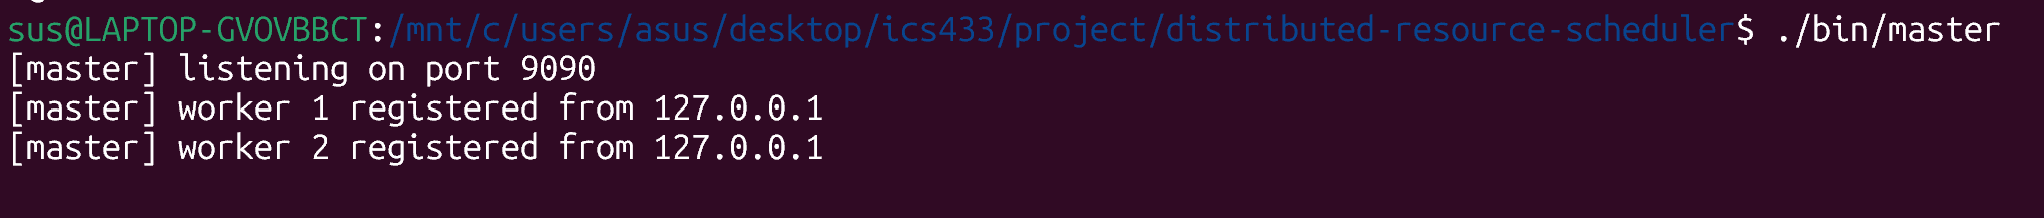
\includegraphics[width=0.85\textwidth]{screenshot_master_startup.png}
\caption{Master node listening and workers registering.}
\end{figure}

\subsection{Task Dispatch and Result Collection}
\begin{figure}[H]
\centering
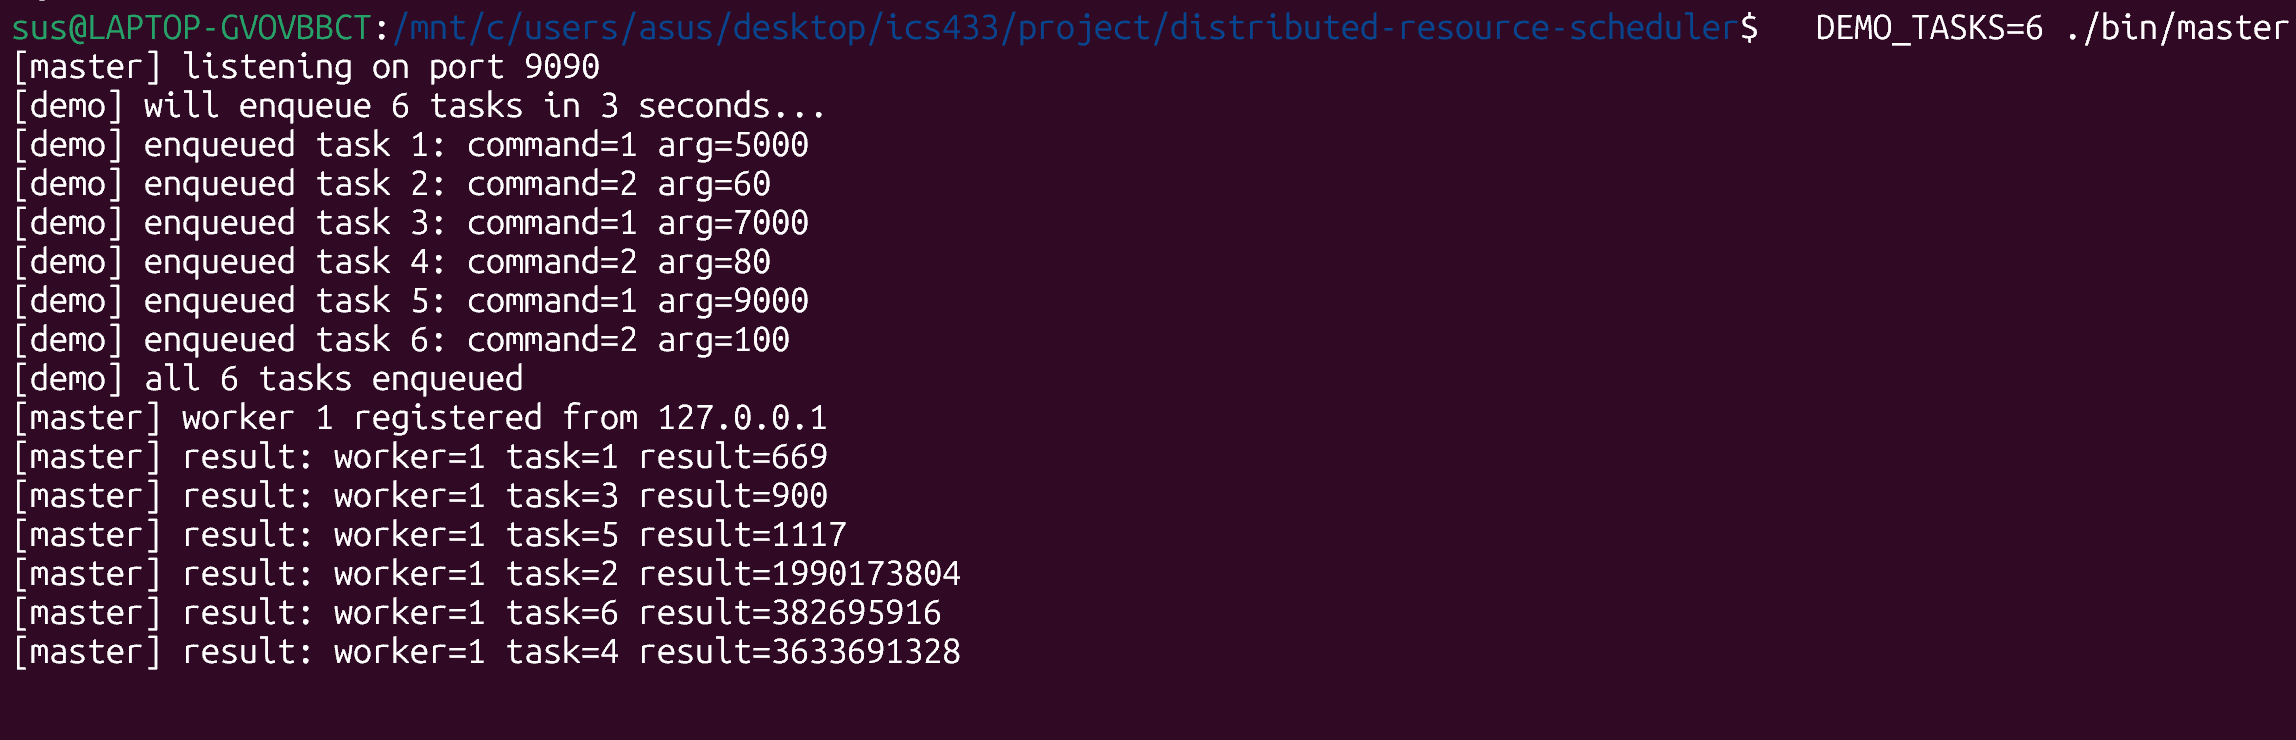
\includegraphics[width=0.85\textwidth]{screenshot_task_dispatch.png}
\caption{Master dispatching tasks and collecting results from workers.}
\end{figure}

\subsection{Worker Node Output}
\begin{figure}[H]
\centering
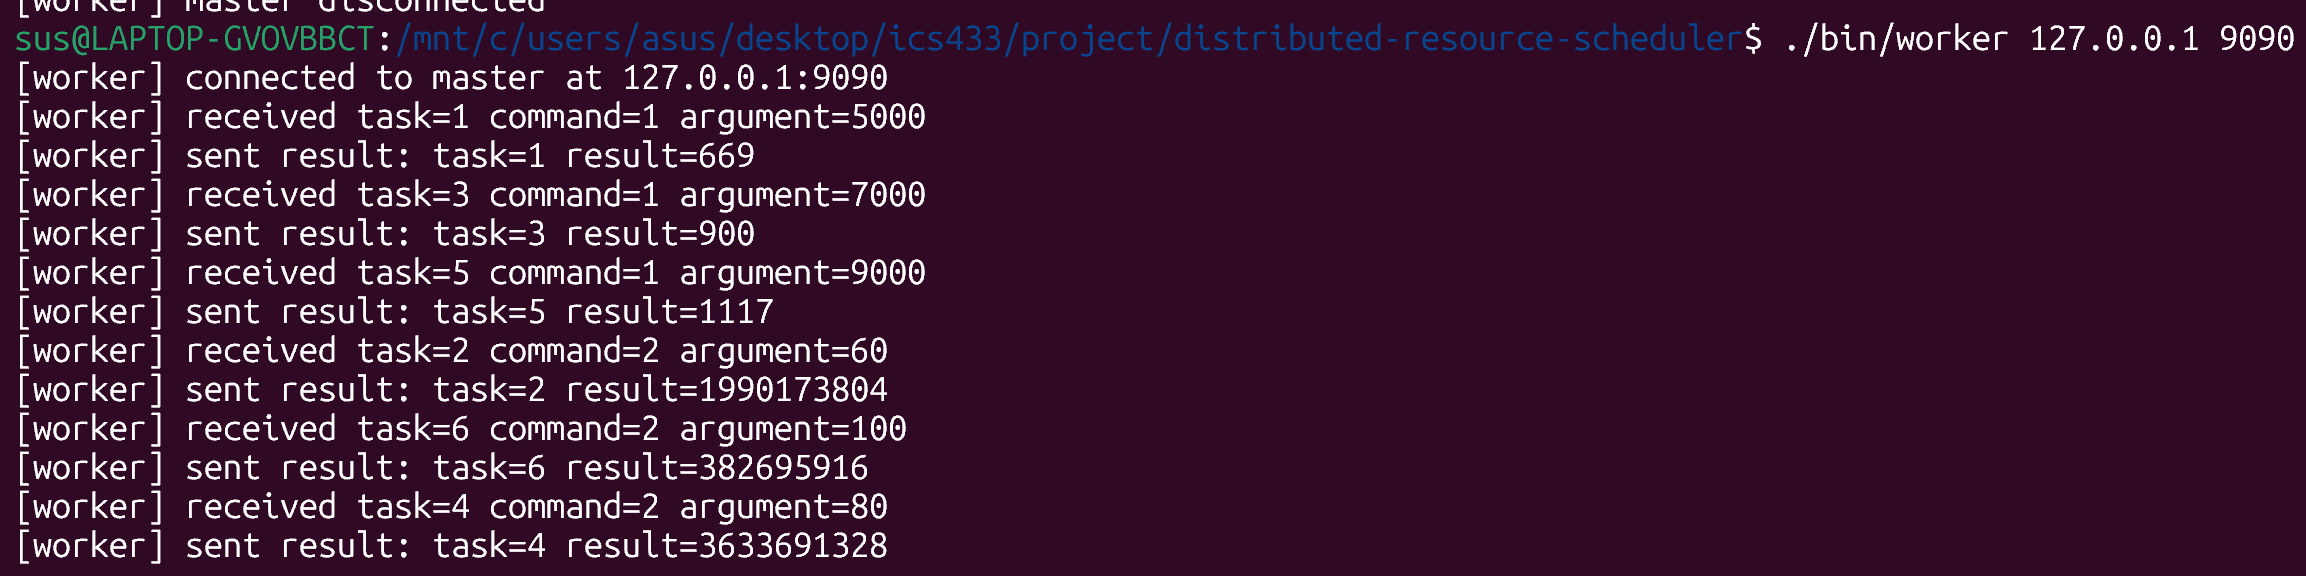
\includegraphics[width=0.85\textwidth]{screenshot_worker_output.png}
\caption{Worker receiving a task, executing it, and sending the result back.}
\end{figure}

\subsection{Unit Test Output}
\begin{figure}[H]
\centering
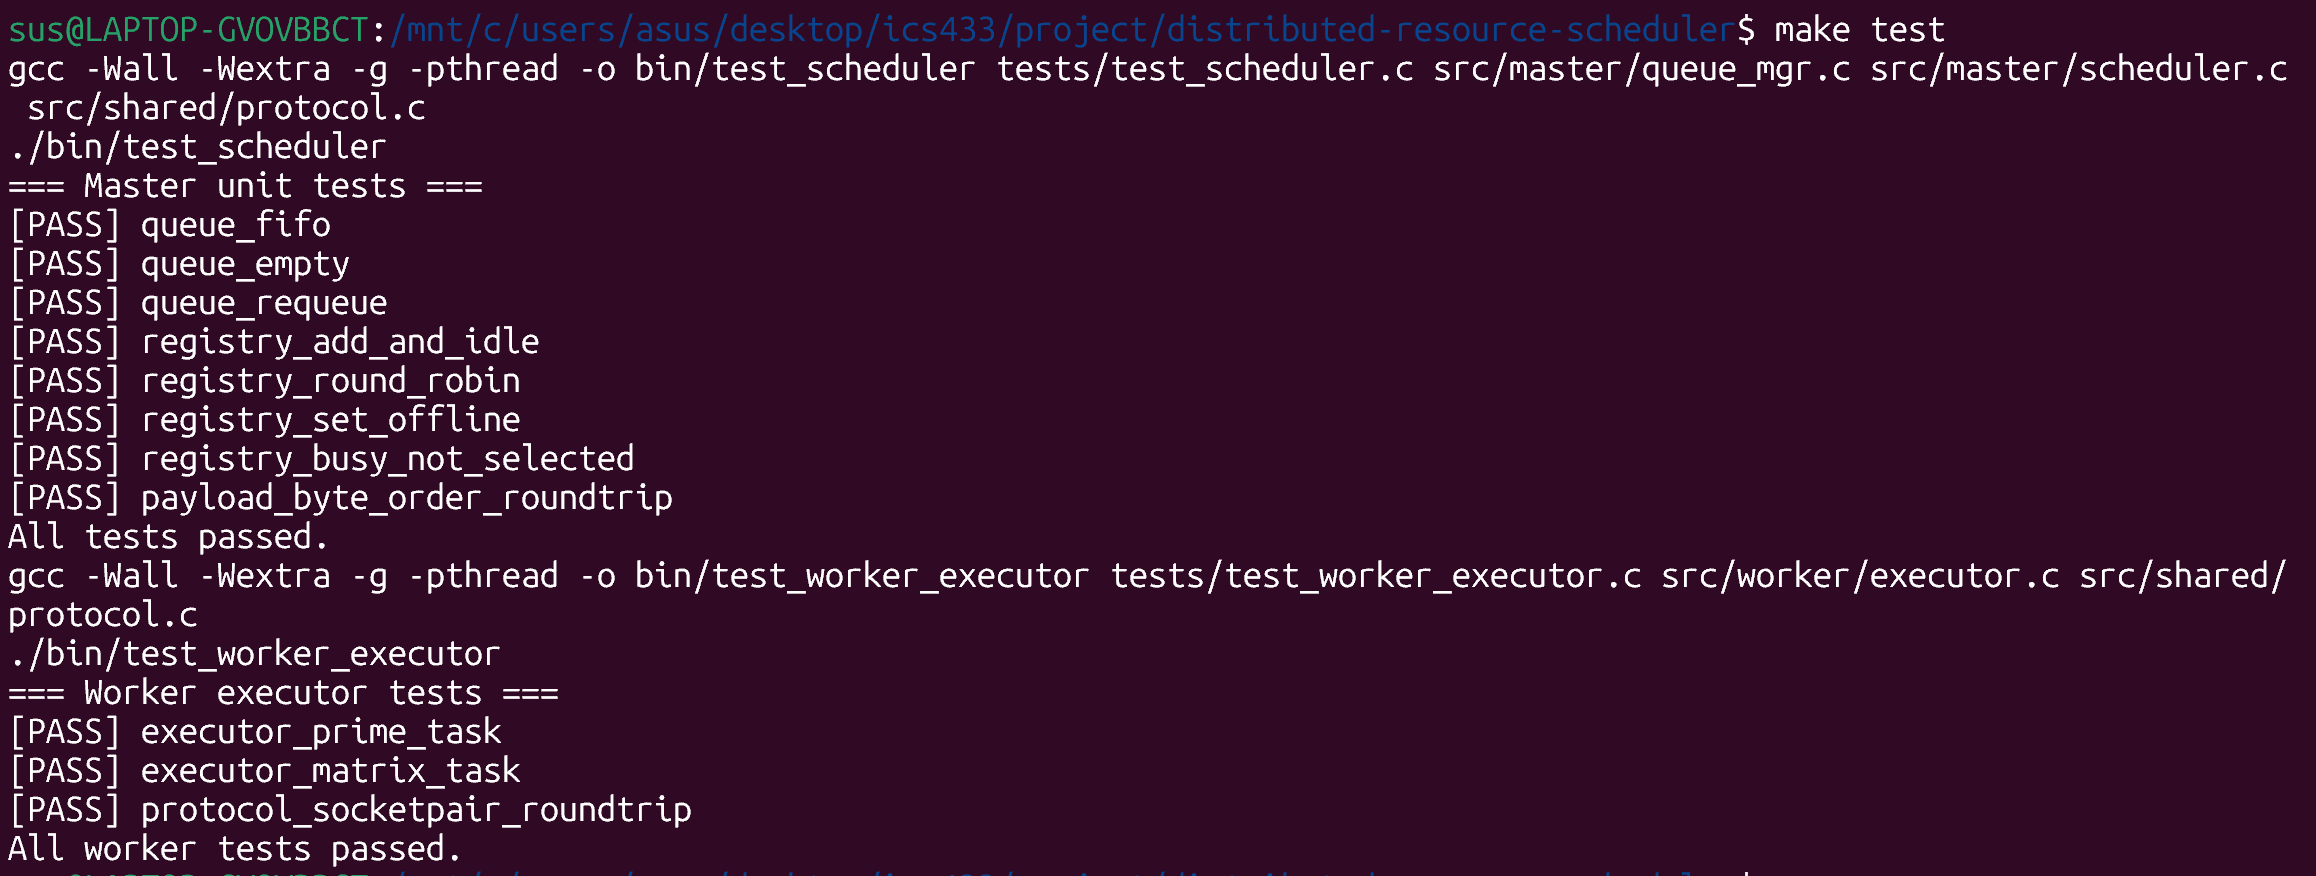
\includegraphics[width=0.85\textwidth]{screenshot_tests.png}
\caption{All unit tests passing (\texttt{make test}).}
\end{figure}

\subsection{Fault Tolerance --- Worker Disconnect and Task Requeue}
\begin{figure}[H]
\centering
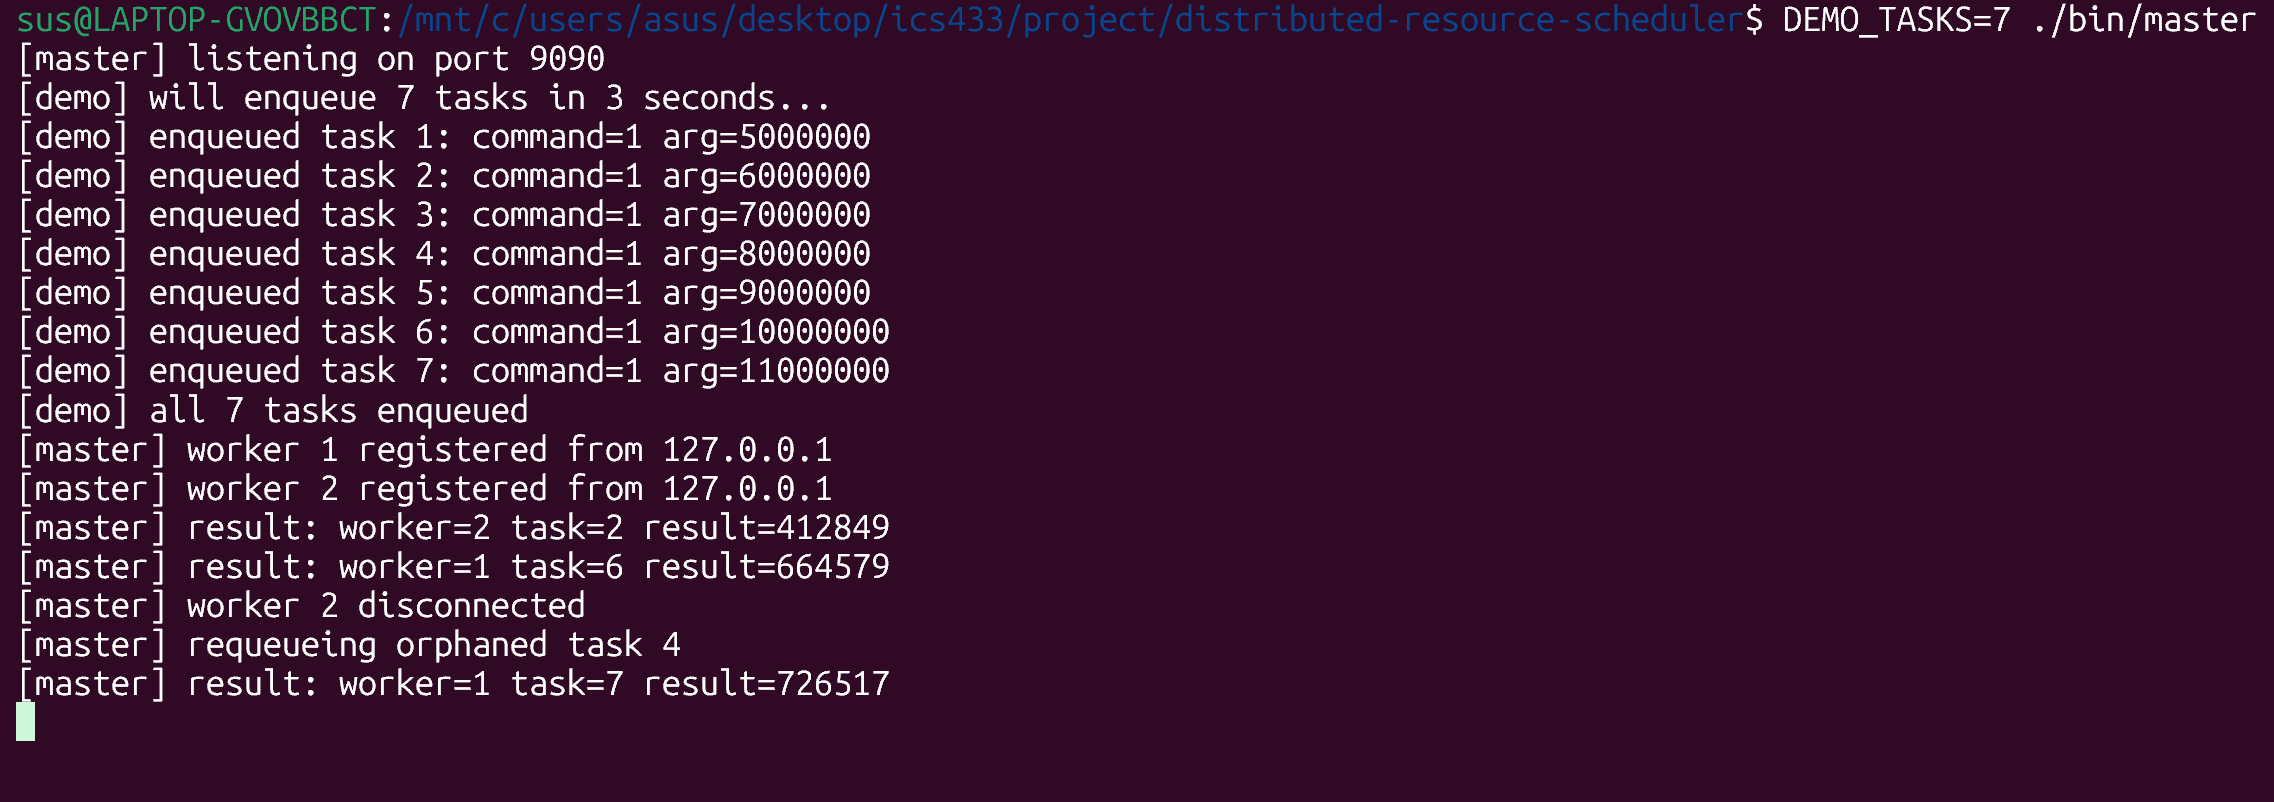
\includegraphics[width=0.85\textwidth]{screenshot_fault_tolerance.png}
\caption{Master detecting worker disconnect and requeueing the orphaned task.}
\end{figure}

% ==============================================================================
\section{How to Run the System}
\label{sec:howtorun}

This section provides the exact commands to run for generating the screenshots
above and for verifying the system works end-to-end.

\subsection{Build}
\begin{lstlisting}[style=shellstyle]
# From the project root:
make all
# Produces: bin/master and bin/worker
\end{lstlisting}

\subsection{Run Unit Tests}
\begin{lstlisting}[style=shellstyle]
make test
# Runs both test suites and prints PASS/FAIL for each case.
# Expected output: "All tests passed."
\end{lstlisting}

To run each suite separately:
\begin{lstlisting}[style=shellstyle]
make test_scheduler      # 8 master unit tests (queue, registry, protocol)
make test_worker         # 3 worker unit tests (prime, matrix, socket roundtrip)
\end{lstlisting}

\subsection{Run Integration Test (Local --- 3 Workers)}
Open \textbf{four terminals}:

\textbf{Terminal 1 --- Start the master with 6 demo tasks:}
\begin{lstlisting}[style=shellstyle]
DEMO_TASKS=6 ./bin/master
\end{lstlisting}

\textbf{Terminals 2, 3, 4 --- Start workers:}
\begin{lstlisting}[style=shellstyle]
./bin/worker 127.0.0.1 9090
\end{lstlisting}

Or use the provided script to start 3 workers at once:
\begin{lstlisting}[style=shellstyle]
./start-workers.sh 3 127.0.0.1 9090
\end{lstlisting}

\subsection{Run with Docker}
\begin{lstlisting}[style=shellstyle]
docker-compose build
./scale_workers.sh 2 1 1    # 2 RPi3 + 1 RPi4 + 1 RPi5 workers
docker-compose logs -f master
\end{lstlisting}

\subsection{Test Fault Tolerance}
\begin{lstlisting}[style=shellstyle]
# 1. Start master with many tasks:
DEMO_TASKS=20 ./bin/master

# 2. Start 3 workers:
./start-workers.sh 3 127.0.0.1 9090

# 3. Wait a few seconds, then kill one worker (Ctrl-C in its terminal).
#    The master terminal should print:
#      [master] worker N disconnected
#      [master] requeueing orphaned task X
#    And the surviving workers should complete all tasks.
\end{lstlisting}

% ==============================================================================
\section{Challenges Faced}

\subsection{Thread Safety Without Deadlock}
The master holds two independent mutexes: \texttt{registry.lock} and \texttt{queue.lock}.
Early versions acquired both simultaneously (from within the scheduler thread), which
risked deadlock when the server thread also needed the registry lock.
The solution was to release \texttt{registry.lock} before calling \texttt{queue\_requeue()},
ensuring the two subsystem locks are never held concurrently.

\subsection{TCP Partial Reads}
A naive single \texttt{recv()} call for a \texttt{NetworkPayload} would silently return fewer
than 24 bytes under load. Both the master and worker now use \texttt{recv\_full()} and
\texttt{send\_full()} --- looping until exactly \texttt{sizeof(NetworkPayload)} bytes have
been transferred --- which eliminated intermittent message corruption.

\subsection{Worker Disconnect Race}
When a worker disconnects, its in-flight task must be requeued exactly once.
The initial implementation could race: the server thread could set the worker offline
before the task snapshot had been captured, losing the task. The fix was to snapshot
\texttt{current\_task} while still holding \texttt{registry.lock}, release the lock,
\emph{then} call \texttt{queue\_requeue()}, with a guard on \texttt{task\_id != 0} to
skip workers that were idle at disconnect time.

\subsection{Child Process Cleanup}
The executor originally leaked zombie processes because the parent \texttt{worker\_run}
loop did not call \texttt{waitpid()}. After moving execution into its own thread and
calling \texttt{waitpid()} inside \texttt{executor\_run\_task()}, child reaping is now
deterministic. Using \texttt{\_exit()} in the child also prevents double-flushing of
parent \texttt{stdio} buffers.

\subsection{Heartbeat and Send Interleaving}
The heartbeat thread and task-result thread both write to the same socket.
Without synchronization, their bytes would interleave, corrupting the master's protocol
parser. A dedicated \texttt{send\_lock} mutex serializes all socket writes from the worker,
regardless of which thread initiates them.

% ==============================================================================
\section{Implementation Progress Summary}

\begin{center}
\begin{tabular}{>{\bfseries}lccl}
\toprule
Module & Status & \% Done & Notes \\
\midrule
TCP Server (\texttt{server.c})         & Complete    & 100\% & Registration, dispatch, disconnect \\
Task Queue (\texttt{queue\_mgr.c})     & Complete    & 100\% & FIFO, requeue, thread-safe \\
Scheduler (\texttt{scheduler.c})       & Complete    & 100\% & Round-robin, fault-safe \\
Worker Registry (\texttt{scheduler.c}) & Complete    & 100\% & Slot reuse, mutex-protected \\
Worker Client (\texttt{client.c})      & Complete    & 100\% & Heartbeat, multi-task, graceful shutdown \\
Executor (\texttt{executor.c})         & Complete    & 100\% & fork+pipe, prime+matrix workloads \\
Protocol Layer (\texttt{protocol.c})   & Complete    & 100\% & Fixed-size, byte-order safe \\
Unit Tests                             & Complete    & 100\% & 11 passing tests \\
Docker / Scripts                       & Complete    & 100\% & Compose, scale, manage scripts \\
Dashboard (\texttt{dashboard.c})       & Stub only   & 0\%   & ncurses UI not yet implemented \\
Remote Code Execution                  & Not started & 0\%   & Dynamic task dispatch from master \\
Raspberry Pi Deployment                & Not started & 0\%   & Real LAN demo (time-permitting) \\
\midrule
\multicolumn{2}{l}{\textbf{Overall}} & \textbf{$\approx$65\%} & \\
\bottomrule
\end{tabular}
\end{center}

% ==============================================================================
\section{Plan for Completing Remaining Work}

\subsection{Remote Code Execution on Workers (Core Priority)}

Currently the executor only supports two hard-coded workloads (prime counting and matrix
checksum). The primary Phase 3 goal is to extend the worker into a general-purpose
\textbf{remote execution engine} that can receive and run arbitrary programs dispatched
by the master.

The planned approach:
\begin{itemize}[noitemsep]
    \item \textbf{Extended protocol:} add a \texttt{MSG\_EXEC} message type that carries a
          command string or binary payload in addition to the existing integer argument.
          The \texttt{NetworkPayload} struct will be extended (or a variable-length framing
          scheme added) to accommodate program names and arguments.
    \item \textbf{Executor extension:} \texttt{executor\_run\_task()} will use \texttt{execvp()}
          in the forked child to replace itself with the target program. The parent continues
          to collect output via the pipe and relay it to the master as a \texttt{MSG\_RESULT}.
    \item \textbf{Security boundary:} only programs present in a whitelist directory on the
          worker will be executed, preventing arbitrary command injection from the master.
    \item \textbf{Output capture:} \texttt{stdout} and \texttt{stderr} of the child process
          will be redirected into the pipe so the master can log full program output, not just
          a single integer result.
\end{itemize}

This change makes the system a genuine distributed compute platform rather than a
fixed-workload simulator.

\subsection{Terminal Dashboard (Mohammed Yar)}

The dashboard stubs in \texttt{src/ui/dashboard.c} need to be replaced with a full
\texttt{ncurses} implementation. The planned layout uses three \texttt{WINDOW} panels:

\begin{itemize}[noitemsep]
    \item \textbf{Top panel} --- live task queue depth (bar chart or counter).
    \item \textbf{Middle panel} --- worker status table: ID, IP address, status, last heartbeat, current task.
    \item \textbf{Bottom panel} --- scrolling log of recent events (task dispatch, results, disconnects).
\end{itemize}

A background \texttt{pthread} will copy a snapshot of the registry under lock every 500\,ms
and call \texttt{wrefresh()} to update the display without blocking the network threads.

\subsection{Heartbeat Watchdog}

The master currently records \texttt{last\_heartbeat} timestamps but does not actively
check them. A watchdog thread should mark workers \texttt{OFFLINE} if no heartbeat has
arrived within a configurable timeout (e.g., $3\times$ the heartbeat interval = 15 seconds),
enabling automatic detection of silently crashed nodes.

\subsection{Result Logging}

Task completion events (worker ID, task ID, command, argument, result, wall-clock latency)
should be written to a CSV log file for post-run performance analysis and graphing in the
final report.

\subsection{Additional Test Coverage}

\begin{itemize}[noitemsep]
    \item \texttt{test\_forking.c} and \texttt{test\_protocol.c} exist in \texttt{tests/} but are not yet wired into the Makefile. These will be completed and integrated into \texttt{make test}.
    \item An end-to-end integration test script will verify task completion count and
          fault-tolerance behavior automatically without manual observation.
    \item Unit tests for the extended \texttt{execvp()}-based executor will be added once
          remote code execution is implemented.
\end{itemize}

\subsection{Raspberry Pi Deployment (Time-Permitting)}

If time permits, the system will be deployed on real hardware to demonstrate a genuine
distributed LAN scenario:

\begin{itemize}[noitemsep]
    \item \textbf{Master node:} the development PC (x86-64, Linux/WSL) runs \texttt{bin/master}.
    \item \textbf{Worker nodes:} one or more Raspberry Pi devices (ARM, Linux) compile and run
          \texttt{bin/worker}, connecting to the PC's LAN IP address.
    \item \textbf{Cross-compilation:} the worker binary will be cross-compiled for ARM using
          \texttt{arm-linux-gnueabihf-gcc}, or compiled natively on each Pi.
    \item \textbf{Demo scenario:} the master dispatches a batch of compute tasks (prime counts,
          matrix checksums, or real programs via remote execution) across the Pi workers. The
          terminal dashboard on the PC shows live worker status, queue depth, and results
          arriving from physically separate machines.
    \item \textbf{Fault tolerance demo:} unplugging a Pi's network cable demonstrates automatic
          task requeue and system recovery in a real environment.
\end{itemize}

This deployment would serve as the capstone demonstration for the final report and
validates that the system works correctly across heterogeneous architectures and a real
network, not just localhost.


% ==============================================================================
\section{Repository Structure}

\begin{lstlisting}[basicstyle=\ttfamily\small, frame=single, backgroundcolor=\color{gray!6}]
distributed-resource-scheduler/
|-- src/
|   |-- master/
|   |   |-- queue_mgr.c / .h     # FIFO task queue
|   |   |-- scheduler.c / .h     # Round-robin scheduler + registry
|   |   +-- server.c / .h        # TCP server + main()
|   |-- worker/
|   |   |-- client.c / .h        # TCP client + heartbeat + main()
|   |   +-- executor.c / .h      # fork()+pipe() execution engine
|   |-- shared/
|   |   |-- models.h             # NetworkPayload, enums
|   |   +-- protocol.c / .h      # recv_full, send_full, byte-order
|   +-- ui/
|       +-- dashboard.c / .h     # ncurses stub (Phase 3)
|-- tests/
|   |-- test_scheduler.c         # 8 master unit tests
|   |-- test_worker_executor.c   # 3 worker unit tests
|   |-- test_forking.c           # (in progress)
|   +-- test_protocol.c          # (in progress)
|-- workloads/
|   |-- prime_calc.c             # Reference workload
|   +-- matrix_math.c            # Reference workload
|-- bin/                         # Compiled binaries
|-- Dockerfile
|-- docker-compose.yml
|-- Makefile
|-- start-workers.sh
|-- scale_workers.sh
|-- manage_workers.sh
+-- README.md
\end{lstlisting}

% ==============================================================================
\end{document}
